\chapter{Quantum mechanics on a computer}
% \begin{itemize}
% \item Descriptions of how to perform simulations of atomic systems and Bose–Einstein condensates. Include numerical methods, interaction pictures, Monte–Carlo wavefunction methods and other acquired wisdom that would be relevant to anyone implementing similar simulations.

% \item Fourier method: usefulness, use with RK4IP, limitations (i.e. first derivs no good near vortices)


% \end{itemize}


%     Operators and their matrix representation
%     The general case: Need to integrate the equations of motion. What does this mean in a computer? Formal solution of the Schrodinger equation. Is not so formal - can be typed into a programming language thusly: [example code - time ordered product of matrix exponentials].

%     Every symbol on the paper has a representation in a computer. State vectors are arrays of complex numbers, operators are matrices - differential operators are no exception. Operators must have a concrete representation, their matrix elements can be computed and then things solved with linear algebra. For discrete degrees of freedom, the matrix representation of the operators may be known, for continuous ones you can find the matrix elements once you define what basis functions you will use [show how]. Or, for the DVR it is a little more subtle (because it's not a basis) but still basically the same process.

% \section{The interaction picture}
%     \begin{itemize}
%         \item Sometimes called a "rotating frame"
%         \item Is equivalent to basis change where new basis functions differ by a time-dependent phase factor
%         \item Is defined by a time-independent Hamiltonian
%         \item This has the effect of moving some time dependence into the operators (demonstrate, by writing some operators with the unitary in front of them. As you can see it is simply a change of basis - but a time-dependent one.)
%         \item No need to remain in the same interaction picture - can be redefined arbitrarily often throughout a simulation and state vectors transformed into new basis.
%     \end{itemize}

% \section{Discrete degrees of freedom}
%     \subsection{Unitary integration}
%         \subsubsection{Direct exponentiation via diagonalisation of Hamiltonian}
%         \begin{itemize}
%         \item Unitary - doesn't mean it's accurate but means it won't explode. Great for the bits of your simulation that are explosion-prone but don't matter (like regions of space where the wavefunction is near zero but the potential is large or steep)
%         \item error is order [whatever it is] per timestep, not great compared to RK4
%         \item can be combined with RK4 to improve accuracy (see later subsection)
%         \end{itemize}
%         \subsubsection{Approximate exponentiation by operator product}

%         [Comment in this section how the approximate total unitary can be used at each timestep to define an interaction picture, and the remaining dynamics simulated with RK4 like RKILIP does in the spatial basis. Interaction pictures are really useful!]
% \section{Continuous degrees of freedom}
%     \begin{itemize}
%         \item Have to be discretised in some way to simulate on a computer - need basis functions. Often a spatial basis is used. Any spatial basis must be combined with assumptions about what the wavefunction is doing at points in between the basis points, in order to define differential operators. Finite differences approximates wavefunction as low-order polynomial in between points (is this equivalent to a polynomial \emph{basis}? Probably not.). Fourier method assume the Fourier series of the wavefunction at the given points can be used to interpolate between points (or the wavefuntion can be Fourier transformed and calculations can be done directly in the Fourier basis). DVR is not actually a spatial basis despite appearances. It assumes the wavefunction is a sum of polynomial 'shape functions', but these shape functions are not basis functions as they are not orthonormal. This is why it is called a representation rather than a basis. Regardless, the shape functions can be used to define an interpolation of the wavefunction between points and thus define differential operators.

%     \end{itemize}
%     \subsection{Finite differences}
%         Show a matrix representation of a few different finite differences, to show that differential operators really are just matrices. They approximate the function as low-order polynomials about each point. You can take them to arbitrarily high order.
%     \subsection{The Fourier basis}
%         Because of properties of Fourier transforms, derivitives can be taken in Fourier space as simple multiplication. This is essentially because differential operators are diagonal in the Fourier basis. So you can use this fact to define a differential operator in the spatial basis [show matrix] ...or, you could just implement it with Fourier transforms, since FFTs are faster than matrix-vector multiplication ($O(n \log (n)$) rather than $O(n^2)$)
%         \subsubsection{Split operator method}
%             \begin{itemize}
%             \item Equivalent to approximate exponentiation via operator product with the discrete case
%             \end{itemize}
%     \subsection{Harmonic oscillator basis functions}

% \section{Finding groundstates}
% \subsection{Imaginary time evolution}
% \subsection{Successive over-relaxation}
% \subsection{Generalisation to excited states via Gram–Schmidt orthonormalisation}
% Directly diagonalising a Hamiltonian can be costly in a spatial basis. Another approach is to find the groundstate using one of the above techniques, and then repeat the process, subtracting off the wavefunction's projection onto the already found groundstate at every step. This yields the lowest energy state that is orthogonal to the first - i.e the first excited state. Repeating the process, but subtracting off \emph{both} eigenstates found so far, then yields the second excited state and so forth. This is simply the Gram-Schmidt process for finding orthonormal vectors, with the additional step of relaxing each vector to the lowest possible energy for each one - this ensures the eigenstates of the Hamiltonian are produced, rather than a different orthogonal basis. Extra conditions can be imposed on the wavefunction at each relaxation step in order to obtain particular solutions in the case of degenerate eigenstates. For example, a phase winding can be imposed in order to obtain a particular harmonic oscillator state - otherwise this process produces an arbitrary superposition of basis states that have equal energy.

% \section{The finite-element discrete variable representation}

% [explanation of how it works, comparison of implementation with RSP4 vs something like RK4. RK4 is more general purpose, method does not need to be modified for different Hamiltonians. Main limitation is inability to factor out fast dynamical phases, see RK4ILIP for solution to this. MPI implementation and scaling properties with increasing cores. Superscaling at low number of cores. Mention how my implementation can tolerate high network latency due to early sending od data before all local computations are complete. Mention that it is ripe for GPU processing. Limitations: vulnerable to Runge's phenomenon for sharp potentials. Can't increase the order of the polynomials much because small spacing at the edges requires tiny timesteps. Possible solution: pre-conditioning the potential to be an approximation better representable in the DVR basis.]

\setcounter{section}{5}
\section{Fourth order Runge--Kutta in an instantaneous local interaction picture}
\sectionmark{RK4 in an instantaneous local interaction picture}

Consider the differential equation for the components of a state vector $\ket{\psi(t)}$ in a particular basis with basis vectors $\ket{n}$. This might simply be the Schr\"odinger equation, or perhaps some sort of nonlinear or other approximate, effective or phenomenological equation not corresponding to pure Hamiltonian evolution. Though they may have additional terms, such equations are generally of the form:
\begin{align}\label{eq:real_imag}
\dv t \braket{n}{\psi(t)} = -\frac i \hbar \sum_m \matrixel{n}{\hat H(t)}{m} \braket{m}{\psi(t)},
\end{align}
where $\matrixel{n}{\hat H(t)}{m}$ are the matrix elements in that basis of the Hamiltonian $\hat H(t)$, which in general can be time dependent, or even a function of $\ket{\psi(t)}$, depending on the exact type of equation in use. Often, and if the basis is chosen well\footnote{That is to say, the basis is close to being an eigenbasis of the Hamiltonian.}, this type of evolution is dominated by simple dynamical phase evolution, that is, $\hat H(t)$ is almost diagonal in the $\ket{n}$ basis. A transformation into an interaction picture (\textsc{ip}) is commonly used to treat this part of the evolution analytically, before solving the remaining dynamics with further analytics or numerics. For numerical methods, integration in the interaction picture allows one to take larger integration timesteps, as one does not need to resolve the fast oscillations around the complex plane due to this dynamical phase.

Choosing an interaction picture typically involves diagonalising the time independent part of a Hamiltonian, and then proceeding in the basis in which that time-independent part is diagonal. However, often one has a good reason to perform computations in a different basis, in which the time independent part of the Hamiltonian is only approximately diagonal\footnote{For example, a spatial basis which allows for partitioning the integration region over multiple nodes on a cluster or cores on a \textsc{gpu}.}, and transforming between bases may be computationally expensive (involving large matrix-vector multiplications). Furthermore, the Hamiltonian may change sufficiently during the time interval being simulated that the original time-independent Hamiltonian to no longer dominates the dynamics at later times. In both these cases it would still be useful to factor out the time-local oscillatory dynamics in whichever basis is being used, in order to not have to take unreasonably small timesteps.

To that end, suppose we decompose $\hat H(t)$ into diagonal and non-diagonal (in the $\ket{n}$ basis) parts at each moment in time:
\begin{align}
\hat H(t) = \hat H_\up{diag}(t) + \hat H_\up{nondiag}(t),
\end{align}
and use the diagonal part at a specific time $t=t^\prime$ to define a time-independent Hamiltonian:
\begin{align}\label{eq:H0def}
 \hat H_0^{t^\prime} = \hat H_\up{diag}(t^\prime),
\end{align}
which is diagonal in the $\ket{n}$ basis. We can then use then use $\hat H_0^{t^\prime}$ to define an interaction picture state vector $\ket{\psi_\up{I} ^{t^\prime}(t)}$:
\begin{align}\label{eq:IP_definition}
\ket{\psi_\up{I}^{t^\prime}(t)} = e^{\frac i \hbar \hat H_0^{t^\prime}(t - t^\prime)}\ket{\psi(t)},
\end{align}
which obeys the differential equation:
\begin{align}\label{eq:IPDE}
\dv t \ket{\psi_\up{I}^{t^\prime}(t)}
    = e^{\frac i \hbar \hat H_0^{t^\prime}(t - t^\prime)}\dv t \ket{\psi(t)}
      + \frac i\hbar \hat H_0^{t^\prime}\ket{\psi_\up{I}^{t^\prime}(t)},
\end{align}
where:
\begin{align}\label{eq:backtransform}
\ket{\psi(t)} = e^{-\frac i \hbar \hat H_0^{t^\prime}(t - t^\prime)}\ket{\psi_\up{I}^{t^\prime}(t)}
\end{align}
is the original Schrödinger picture (\textsc{sp}) state vector.

This transformation is exact, no approximations or assumptions have been made. If indeed the dynamics of $\ket{\psi(t)}$ in the given basis are dominated by fast oscillating dynamical phases, then solving the differential equation \eqref{eq:IPDE} for $\ket{\psi_\up{I}^{t^\prime}(t)}$ should allow one to take larger integration timesteps than solving \eqref{eq:real_imag} directly. And if not, then it should do no harm other than the (small) computational costs of computing some extra exponentials.

Equation \eqref{eq:IP_definition} defines an \emph{instantaneous} interaction picture, in that it depends on the dynamics at a specific time $t=t^\prime$, and can be recomputed repeatedly throughout a computation in order to factor out the fast dynamical phase evolution even as the oscillation rates change over time. It is \emph{local} in that $H_0^{t^\prime}$ is diagonal in the $\ket{n}$ basis, which means that transformations between Schrödinger picture and interaction picture state vectors involves ordinary elementwise exponentiation of vectors, rather than matrix products. Thus \eqref{eq:IP_definition}, \eqref{eq:IPDE} and \eqref{eq:backtransform} can be written componentwise as:

\begin{align}\label{eq:IP_definition_components}
\braket{n}{\psi_\up{I}^{t^\prime}(t)} = e^{ i \omega_n^{t^\prime}(t - t^\prime)}\braket{n}{\psi(t)},
\end{align}
\begin{align}\label{eq:IPDE_components}
\dv t \braket{n}{\psi_\up{I}^{t^\prime}(t)}
    = e^{i \omega_n^{t^\prime}(t - t^\prime)}\dv t \braket{n}{\psi(t)}
      + i\omega_n^{t^\prime}\braket{n}{\psi_\up{I}^{t^\prime}(t)},
\end{align}
and:
\begin{align}\label{eq:backtransform_components}
\braket{n}{\psi(t)} = e^{-\omega_n^{t^\prime}(t - t^\prime)}\braket{n}{\psi_\up{I}^{t^\prime}(t)},
\end{align}
where we have defined:
\begin{align}\label{eq:omega}
\omega_n^{t^\prime} = \frac 1\hbar \matrixel{n}{\hat H_0^{t^\prime}}{n}
\end{align}
This is in contrast to fourth order Runge--Kutta in the interaction picture (\textsc{rk4ip}) \cite{caradoc_davies_thesis}, in which the interaction picture uses the Fourier basis and thus transforming to and from it involves fast Fourier transforms. \textsc{rk4ip} was developed to augment computations in which \textsc{fft}s were already in use for evaluating spatial derivatives, and so its use of \textsc{fft}s imposes no additional cost. Even if one is using \textsc{fft}s already, our method is still useful for avoiding fast oscillating dynamical phases that are not due to the kinetic term (which is the term of the Hamiltonian that \textsc{rk4ip} takes as its $\hat H_0$). We compare results of the two methods below.

\subsection{Algorithm}
My idea is to use \eqref{eq:IP_definition} to define a new interaction picture at the beginning of each fourth-order Runge–Kutta (\textsc{rk4}) integration timestep. The differential equation and initial conditions supplied to the algorithm are in the ordinary Schr\"odinger picture, and the interaction picture is used only within a timestep, with the Schrödinger picture state vector returned at the end of each timestep. Thus differential equations need not be modified in any way compared to if ordinary \textsc{rk4} were being used, and the only modification to calling code required is for a function to compute and return $\omega_n^{t^\prime}$ be provided.

By being based on fourth order Runge--Kutta integration, this new method enjoys all the same benefits as a workhorse method that is time-proven, and---as evidenced by its extremely widespread use---at a sweet-spot of ease of implementation, accuracy and required computing power.

Below is the resulting algorithm for performing one integration timestep. It takes as input the time $t_0$ at the start of the timestep, the timestep size $\upDelta t$, the components $\psi_0^{(n)}$ of the state vector at the start of the timestep, a function $F(t, \psi^{(n)})$ which takes a time and (the components of) a state vector and returns the time derivative for each component, and a function $G(t, \psi^{(n)})$ which takes the same inputs and returns the interaction picture oscillation frequency $\omega^{(n)}$ for each component at a particular time.

For example, for the case of the Gross-Pitaevskii equation in the spatial basis $\psi(\vec r, t) = \braket{\vec r}{\psi(t)}$, these would be:
\begin{align}\label{eq:RK4_ILIP_GPE}
F(t, \psi(\vec r, t)) = -\frac i \hbar\left[-\frac{\hbar^2}{2m}\nabla^2 + V(\vec r, t) + g|\psi(\vec r, t)|^2\right]\psi(\vec r, t),
\end{align}
and
\begin{align}
G(t, \psi(\vec r, t)) = \frac1\hbar\left[V(\vec r, t) + g|\psi(\vec r, t)|^2\right].
\end{align}

Note that each symbol with a superscript $^{(n)}$ denotes the entire set over all $n$, subscripts denote the different stages of \textsc{rk4}, and all operations are elementwise. The only opportunity for non-elementwise operations to occur is within $F$, which contains the details of any couplings between basis states for whatever system of equations is being solved, for example, using \textsc{fft}s or finite differences to evaluate the Laplacian in \eqref{eq:RK4_ILIP_GPE}.


\begin{breakablealgorithm}
    \caption{\textsc{rk4ilip}}
    \begin{algorithmic}[1]
    \linespread{1.5}
    \footnotesize
    \Function{$\up{RK4ILIP}$}{$t_0$, $\upDelta t$, $\psi_0^{(n)}$, $F$}
        \State $f_1^{(n)} \gets F(t_0, \psi_0^{(n)})$
        \Comment{First evaluation of Schrödinger picture DE}
        \State $\omega^{(n)} \gets G(t_0, \psi_0^{(n)})$
        \Comment{Oscillation frequencies: $\hbar\omega^{(n)} = \matrixel{n}{\hat H_\up{diag}(t_0)}{n}$}
        \State $k_1^{(n)} \gets f_1^{(n)} + i\omega^{(n)}\psi_0^{(n)}$
        \Comment{Evaluate \eqref{eq:IPDE_components} with $t-t^\prime=0$}
        \State $\phi_1^{(n)} \gets \psi_0^{(n)} + k_1^{(n)} \frac{\upDelta t}{2}$
        \Comment{First RK4 estimate of IP state vector, at $t=t_0 + \frac{\upDelta t}{2}$}
        \State $\psi_1^{(n)} \gets e^{-i\omega^{(n)}\frac{\upDelta t}{2}}\phi_1^{(n)}$
        \Comment{Convert first estimate back to SP with \eqref{eq:backtransform_components}}
        \State $f_2^{(n)} \gets F(t_0 + \frac{\upDelta t}{2}, \psi_1^{(n)})$
        \Comment{Second evaluation of Schrödinger picture DE}
        \State $k_2^{(n)} \gets e^{i\omega^{(n)}\frac{\upDelta t}{2}}f_2^{(n)} + i\omega^{(n)}\phi_1^{(n)}$
        \Comment{Evaluate \eqref{eq:IPDE_components} with $t-t^\prime=\frac{\upDelta t}{2}$}
        \State $\phi_2^{(n)} \gets \psi_0^{(n)} + k_2^{(n)} \frac{\upDelta t}{2}$
        \Comment{Second RK4 estimate of IP state vector, at $t=t_0 + \frac{\upDelta t}{2}$}
        \State $\psi_2^{(n)} \gets e^{-i\omega^{(n)}\frac{\upDelta t}{2}}\phi_2^{(n)}$
        \Comment{Convert second estimate back to SP with \eqref{eq:backtransform_components}}
        \State $f_3^{(n)} \gets F(t_0 + \frac{\upDelta t}{2}, \psi_2^{(n)})$
        \Comment{Third evaluation of Schrödinger picture DE}
        \State $k_3^{(n)} \gets e^{i\omega^{(n)}\frac{\upDelta t}{2}}f_3^{(n)} + i\omega^{(n)}\phi_2^{(n)}$
        \Comment{Evaluate \eqref{eq:IPDE_components} with $t-t^\prime=\frac{\upDelta t}{2}$}
        \State $\phi_3^{(n)} \gets \psi_0^{(n)} + k_3^{(n)} \upDelta t$
        \Comment{Third RK4 estimate of IP state vector, at $t=t_0 + \upDelta t$}
        \State $\psi_3^{(n)} \gets e^{-i\omega^{(n)}\upDelta t}\phi_3^{(n)}$
        \Comment{Convert third estimate back to SP with \eqref{eq:backtransform_components}}
        \State $f_4^{(n)} \gets F(t_0 + \upDelta t, \psi_3^{(n)})$
        \Comment{Fourth evaluation of Schrödinger picture DE}
        \State $k_4^{(n)} \gets e^{i\omega^{(n)}\upDelta t}f_4^{(n)} + i\omega^{(n)}\phi_3^{(n)}$
        \Comment{Evaluate \eqref{eq:IPDE_components} with $t-t^\prime=\upDelta t$}
        \State $\phi_4^{(n)} \gets
                \psi_0^{(n)} + \frac{\upDelta t}{6}\left(k_1^{(n)} + 2k_2^{(n)} + 2k_3^{(n)} + k_4^{(n)}\right)$
        \Comment{Fourth RK4 estimate, at $t=t_0 + \upDelta t$}
        \State $\psi_4^{(n)} \gets e^{-i\omega^{(n)}\upDelta t}\phi_4^{(n)}$
        \Comment{Convert fourth estimate back to SP with \eqref{eq:backtransform_components}}
        \State \Return $\psi_4^{(n)}$
        \Comment{Return the computed SP state vector at $t=t_0 + \upDelta t$}
    \EndFunction
    \end{algorithmic}
\end{breakablealgorithm}

\subsubsection{Note on imaginary time evolution}

When \textsc{rk4ilip} is used for imaginary time evolution (\textsc{ite}), the oscillation frequencies $\omega_n^{t^\prime}$ may have a large imaginary part. If the initial guess is different enough from the groundstate, then the exponentials in \eqref{eq:IP_definition_components}, \eqref{eq:IPDE_components} and \eqref{eq:backtransform_components} may result in numerical overflow. To prevent this, one can define a clipped copy $\omega^{t^\prime}_\up{clipped}$ of $\omega_n^{t^\prime}$ such that $\abs*{e^{\pm i\omega^{t^\prime}_\up{clipped}\upDelta t}}$ is much less than the largest representable floating point number, and use $\omega^{t^\prime}_\up{clipped}$ in the exponents instead. In the below results I used \textsc{rk4ilip} with \textsc{ite} to smooth initial states after a phase printing, and performed clipping such that\footnote{$400$ being about half the largest (base $e$) exponent representable in double precision floating point.} {$\abs*{\im{(\omega^{t^\prime}_\up{clipped})}\upDelta t} < 400$}. This clipped version of $\omega_n^{t^\prime}$ should be used in all exponents in the above algorithm, but not in the second term of \eqref{eq:IPDE_components}. If it is used everywhere then all we have achieved is to choose a different (less useful) interaction picture, and will still overflow. What we achieve by clipping only the exponents is to have temporarily ``incorrect" evolution\footnote{Of no concern since we are using \textsc{ite} as a relaxation method, and are not interested in intermediate states. Only the final state's correctness concerns us.}, limiting the change in magnitude of each component of the state vector to a factor of $e^{400}$ per step. This will continue for the few steps that it takes \textsc{ite} to get the wavefunction within a factor of $e^{400}$ of the groundstate, after which no clipping is necessary and convergence to the groundstate proceeds as normal, subject to the ordinary limitations on which timesteps may be used with \textsc{ite}.

\subsection{Domain of improvement over other methods}

 For simulations in the spatial basis, \textsc{rk4ilip} treats the spatially local part of the Hamiltonian analytically to first order, and hence can handle larger potentials than ordinary \textsc{rk4}. However, since a global energy offset can be applied to any potential with no physically meaningful change in the results, ordinary \textsc{rk4} can also handle large potentials --- if they are large due a a large constant term which can simply be subtracted off.

So \textsc{rk4ilip} is only of benefit in the case of large \emph{spatial variation} in the potential. Only one constant can be subtracted off potentials without changing the physics --- subtracting a spatially varying potential would require modification of the differential equation in the manner of a gauge transformation in order to leave the system physically unchanged\footnote{Though a numerical solution based on analytically gauging away potentials at each timestep might be equally as fruitful as \textsc{rk4ilip}.}.

However that's not quite all: large spatial variation in potentials often comes with the prospect of the potential energy turning into kinetic energy, in which case \textsc{rk4ilip} is also of little benefit, since in order to resolve the dynamical phase due to the large kinetic term it would have to take timesteps just as small  as ordinary \textsc{rk4} would in order to resolve the dynamical phase evolution from the large potential term.

This leaves \textsc{rk4ilip} with an advantage only in the case of large spatial variations in the potential that cannot lead to equally large kinetic energies. Hence the examples I show in the next section are ones in which the condensate is trapped in a steep potential well --- the trap walls are high and hence involve large potentials compared to the interior, but do not lead to large kinetic energies because the condensate is trapped close to its groundstate.

The Fourier split-step (\textsc{fss}) method (see section [TODO REF TO EARLIER NUMERICS SEC]) also models dynamical phases due to the potential analytically to first order. As such it is also quite capable of modeling large potentials. However, it requires that all operators be diagonal in either the spatial basis or the Fourier basis. Therefore \textsc{bec}s in rotating frames, due to the Hamiltonian containing an angular momentum operator, are not amenable to simulation with \textsc{fss}\footnote{Split step with more than these two bases is possible in other schemes such as \textsc{FEDVR} [TODO SEE EARLIER SECTION] however - each operator can be diagonalised and exponentiated locally in each element and applied as a (relatively small) matrix multiplication rather than using \textsc{fft}s.}.

This use of \textsc{fft}s in both the \textsc{fss} and \textsc{rk4ip} methods necessarily imposes periodic boundary conditions on a simulation, which may not be desired. By contrast, if different boundary conditions are desired, finite differences instead of \textsc{fft}s can be used to evaluate spatial derivatives in the \textsc{rk4} and \textsc{rk4ilip} methods. Finite differences seem to have waned in popularity in \textsc{bec} simulations due to the ``infinite order" accuracy of using \textsc{fft}s for derivatives, but from what I can gather the impression that finite differences are inaccurate stems from only considering second order finite differences [cite FEDVR paper]. As shown in [TODO CITE EARLIER SECTION], 6th or so order finite differences are entirely sufficient for \textsc{bec} simulations.

Along with the ability to impose arbitrary boundary conditions, finite differences require only local data, that is, only points spatially close to the point being considered need be known in order to evaluate derivatives there. This makes finite differences amenable to simulation on cluster computers, with only a small number of points (depending on the order of the scheme) needing to be exchanged at node-boundaries each step. By contrast, \textsc{fft} based derivatives require data from the entire spatial region. Whilst this can still be parallelised on a \textsc{gpu}, where all the data is available, it cannot be done on a cluster without large amounts of data transfer between nodes.

\begin{table}
\centering
\begin{tabular}[c]{|r||rrrr|}
\hline
Method & \textsc{rk4} & \textsc{rk4ip} & \textsc{rk4ilip} & \textsc{fss} \\
\hline
Error & $\Ord{\upDelta t^4}$ & $\Ord{\upDelta t^4}$& $\Ord{\upDelta t^4}$ & $\Ord{\upDelta t^2}$\\
\textsc{fft}s per step & $4$ & $4$ & $4$ & $2$\\
Large $\upDelta V$ & No & No & Yes & Yes\\
Large kinetic term & No & Yes & No & Yes\\
Arbitrary operators & Yes & Yes$^\dagger$ & Yes & No\\
Locally parallelisable & Yes & No & Yes & No\\
Arbitrary boundary conditions & Yes & No & Yes & No\\
\hline
\end{tabular}
\caption{Advantages and disadvantages of four timestepping methods for simulating Bose--Einstein condensates. \emph{Arbitrary operators} refers to whether the method permits operators that are not diagonal in either the spatial or Fourier basis, such as angular momentum operators. \emph{Locally parallelisable} means the method can be formulated so as to use only spatially nearby points in evaluating operators, and thus is amenable to parallelisation by splitting the simulation over multiple cores in the spatial basis.
$\dagger$ Whilst one can include arbitrary operators within the \textsc{rk4ip} method, only operators diagonal in Fourier space can be analytically treated the way \textsc{rk4ip} treats the kinetic term, and so there is no advantage for these terms over ordinary \textsc{rk4}.}\label{table:rk4ilip_methods}
\end{table}

\tableref{table:rk4ilip_methods} summarises the capabilities of the methods considered in the following results section. \textsc{rk4ilip} is the only method capable of modelling a large spatial variation in the potential term whilst being locally parallelisable, and supporting arbitrary operators and boundary conditions.

\subsection{Results}

\afterpage{
    \newgeometry{left=1in,bottom=1.5in,right=1in,top=1.5in}
    \begin{figure}[t]
        \centerfloat
        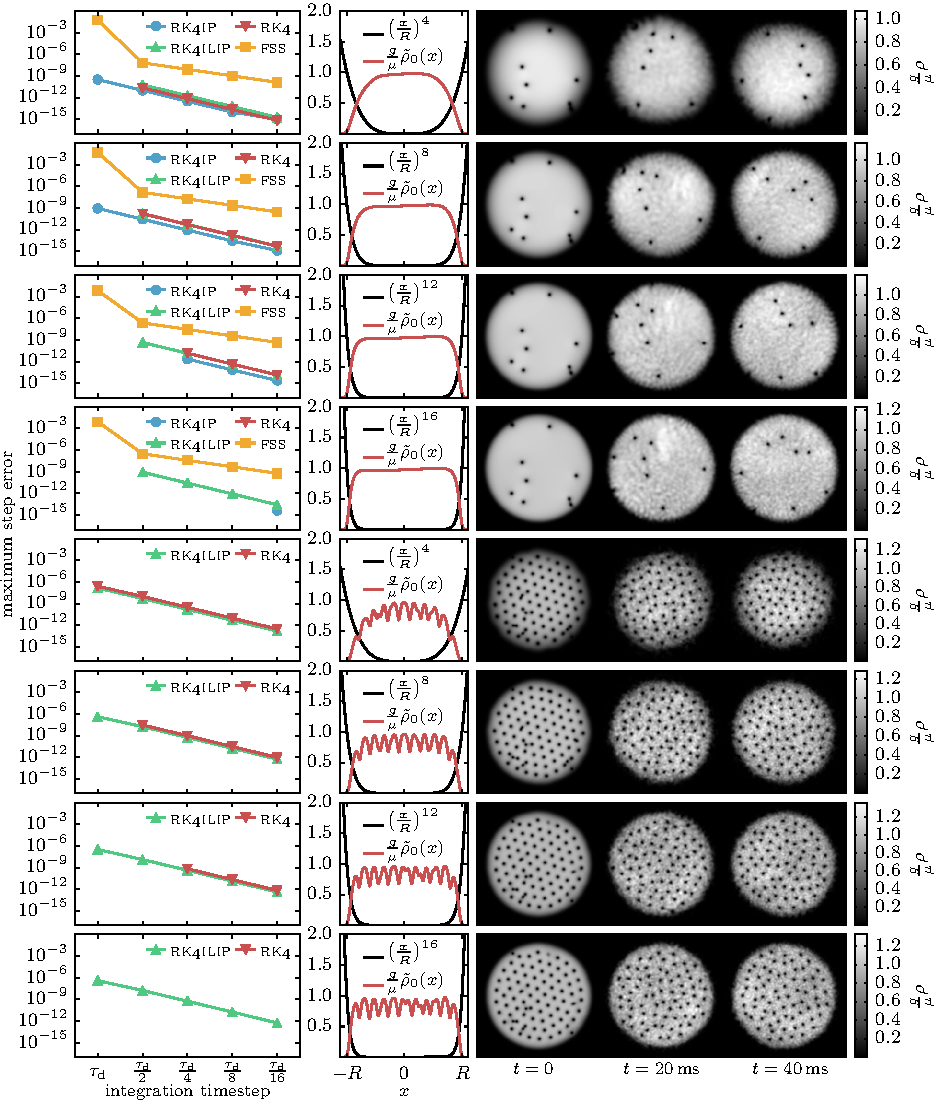
\includegraphics{figures/numerics/rk4ilip_results.pdf}
        \caption{Caption}
        \label{fig:rk4ilip_results}
    \end{figure}
    \restoregeometry
}

 Here I compare four numerical methods: Fourier split-step (\textsc{fss}), fourth order Runge--Kutta in the interaction picture (\textsc{rk4ip}), ordinary fourth order Runge--Kutta (\textsc{rk4}), and my new method --- fourth order Runge--Kutta in an instananeous local interaction picture (\textsc{rk4ilip}).

 The example chosen is a \textsc{2d} simulation of a turbulent Bose--Einstein condensate, in both a rotating and nonrotating frame. For the nonrotating frame the differential equation was as in \eqref{eq:RK4_ILIP_GPE}, and for the rotating frame the same with an additional two terms:
\begin{align}
\hat H_\up{rot} &= -\vec \Omega \cdot \hat{\vec L} +\frac12\hbar m^2\Omega^2 r^2\\
                &= i\hbar\Omega \left(x\pdv{y} - y\pdv{x}\right) +\frac12\hbar m^2\Omega^2 r^2.
\end{align}
The first term is due to the rotating frame, and the second is a harmonic potential to exactly cancel out the resulting centrifugal force. In this way the only potential in the rotating frame is the applied trapping potential.

 Four trapping potentials are used, all radial power laws with different powers. These examples were chosen to demonstrate the specific situation in which \textsc{rk4ilip} provides a benefit over the other methods for spatial Schr\"odinger-like equations.

The results of $120$ simulation runs are shown in \figref{fig:rk4ilip_results}. Each simulation is of $\ ^\up{87}$Rb in the $\ket{F=2, m_F=2}$ state, in which the two-body scattering length is $a = 98.98$ Bohr radii. The simulation region is $20\unit{\mu m}$ in the $x$ and $y$ directions, and the Thomas--Fermi radius is $R = 9\unit{\mu m}$.  The chemical potential is $\mu = 2\pi\hbar\times 1.91\unit{kHz}$, which is equivalent to a maximum Thomas--Fermi density $\rho_\up{max} = 2.5\E{14}\unit{cm}^{-3}$ and a healing length $\xi = 1.1\unit{\mu m}$. There are $256$ simulation grid points in each spatial dimension, which is $14$ points per healing length. The dispersion timescale\footnote{As determined by the phase velocity of the Nyquist mode---see section [TODO REF TO EARLIER SECTION ON NUMERICS]} associated with this grid spacing is $\tau_\up d = 2.68\unit{\mu s}$.

For each simulation, five different timesteps are used: $\upDelta t = \tau_\up d, \frac {\tau_\up d} 2, \frac {\tau_\up d} 4, \frac {\tau_\up d} 8, \frac {\tau_\up d } {16}$. Four different potentials are used, all of the form $V(r) = \mu \left(\frac r R\right)^\alpha$ with $\alpha = 4, 8, 12, 16$. For the rotating frame simulations, the rotation frequency was $\Omega = 2\pi \times 148\unit{Hz}$. This is $89\%$ of the effective harmonic trap frequency, defined as the frequency of the harmonic trap that would have the same Thomas--Fermi radius given the same chemical potential. In addition to the power law potential $V(r)$ used, a harmonic potential of frequency $\Omega$ is also applied to the rotating frame simulations so as to exactly cancel out the centrifugal potential.

All groundstates were determined using with successive over-relaxation [TODO SEE EARLIER SECTION] with sixth-order finite differences for spatial derivatives. For the nonrotating simulations, convergence was reached with $\frac{\upDelta\mu}{\mu} < 1\E{-13}$, with:
\begin{equation}
\upDelta\mu = \sqrt{\frac{\matrixel{\psi} {(\hat H - \mu)^2}{\psi}}{\braket {\psi}{\psi}}},
\end{equation}
where $\hat H$ is the nonlinear Hamiltonian and $\braket{\vec r}{\psi}$ the condensate wavefunction, which does not have unit norm. For the rotating frame simulations the groundstates converged to $\frac{\upDelta\mu}{\mu} \approx 9\E{-7}, 2\E{-6}, 3\E{-6}$ and $2\E{-6}$ for $\alpha = 16, 12, 8$, and $4$ respectively.

After the groundstates were found

[40ms TIME EVOLUTION, FFTs for nonrotating, FD for rotating]

[TODO PAST TENSE]

\subsection{Discussion}

As mentioned, \textsc{rk4ilip} is mostly useful for continuum quantum mechanics only when there are large spatial differences in the potential, which cannot give rise to equally large kinetic energies\footnote{This is essentially due to such a situation violating the condition we laid out at the beginning of this section --- that the simulation basis must be nearly an eigenbasis of the total Hamiltonian.}. Furthermore, the advantage that \textsc{rk4ilip} has over other methods with that same property is that it is does not require a particular form of Hamiltonian or a particular method of evaluating spatial derivatives. The former means is is applicable in rotating frames or to situations with unusual Hamiltonians, and the latter means is can be used with finite differences or \textsc{fedv} and thus is amenable to parallelisation on a cluster computer.

The ability to model a large $\Delta V$ provides only a narrow domain of increased usefulness over other methods. If a large kinetic energy results from the large potential, then the method requires just as small timesteps as any other. And if the large potential is supposed to approximate an an infinite well, then an actual infinite well may be modelled using zero boundary conditions, negating the need for something like \textsc{rk4ilip}. However, when potential wells are steep, but not infinitely steep, \textsc{rk4ilip} provides a benefit. The only other model that can handle these large potentials, Fourier split-step has the disadvantage that it cannot deal with arbitrary operators such as those arising from a rotating frame, and is not parallelisable with local data. The benefits of parallelisability are obvious, and in the previous results I demonstrated \textsc{rk4ilip}'s advantage at simulating \textsc{bec}s in tight traps and rotating frames---\textsc{rk4ilip} was the last method standing.
